\chapter{Anforderungen}
\label{chap:requirements}

\section{Use Cases}
Die funktionalen Anforderungen werden in diesem Kapitel mit Use Cases beschrieben.

\begin{figure}[H]
	\centering
		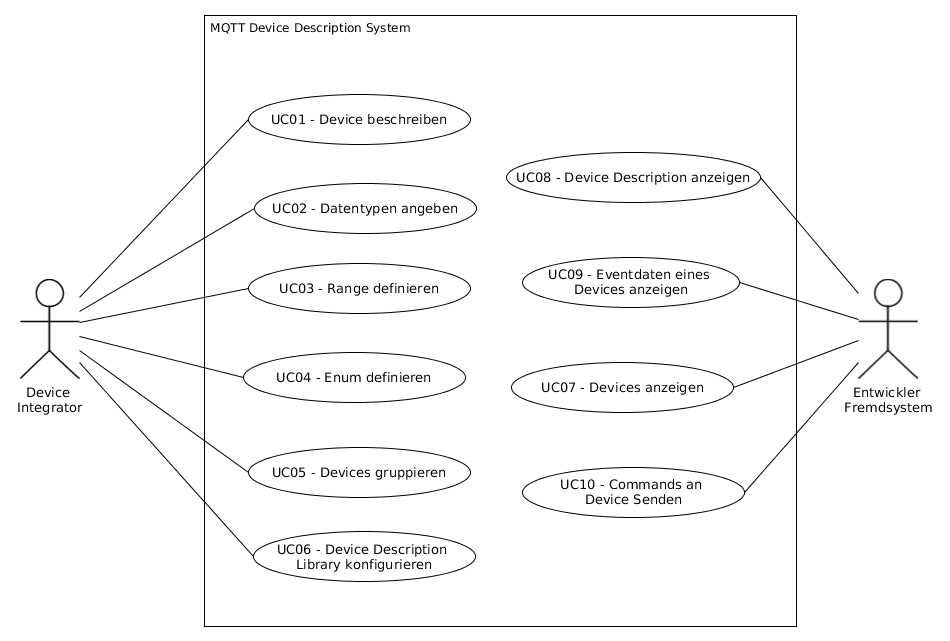
\includegraphics[width=0.9\textwidth]{diag/use_cases.png}
	\caption{Use Case Diagramm}
\end{figure}
\textbf{Aktoren} \\
In den Use Case Beschreibungen werden die folgenden Aktoren als Benutzer des Systems verwendet:

\NumTabs{4}
Device Integrator: Erstellt die Descriptions für seine Devices und integriert die MQTT Device Description Library. \\
Entwickler Fremdsystem: Möchte eine Applikation entwickeln, welche mit den Devices interagiert. \\

\subsection{UC01 - Device beschreiben}

\begin{table}[H]
\begin{tabularx}{\textwidth}{|l|X|}

 \hline
 {\bf Use Case ID }    & UC01 - Device beschreiben \\  \hline
 {\bf Beschreibung }   & In einem Schema müssen die Metadaten der Status- Event- und Commandinformationen aufgeführt werden können.
 \\ \hline
 {\bf Aktor }          & Device Integrator \\ \hline
 {\bf Auslöser }       & Device Description wird erstellt \\ \hline
 {\bf Vorbedingungen } & Funktionalität des Devices ist bekannt \\ \hline
 {\bf Ablauf }         & 
     1. Benutzer erstellt Beschreibung des Device mit der Java MQTT Device Description Library oder manuell \newline                                             
     2. Die Anwendung published die Description des Devices als retained MQTT Message.  \\ \hline
 {\bf Nachbedingungen} & Die Device Description ist auf dem MQTT Broker hinterlegt und kann abgefragt werden. \\ \hline
  
\end{tabularx}
\caption{UC01: Beschreibung Device}
\end{table}

\subsection{UC02 - Datentypen angeben}

\begin{table}[H]
\begin{tabularx}{\textwidth}{|l|X|}

 \hline
 {\bf Use Case ID }    & UC02 - Datentypen angeben \\  \hline
 {\bf Beschreibung }   & Für die State- Event- und Commandangeben muss definiert werden können, welche Datentypen die Werte aufweisen. \\ \hline
 {\bf Aktor }          & Device Integrator \\ \hline
 {\bf Auslöser }       & Device Description wird erstellt. \\ \hline
 {\bf Vorbedingungen } & \gls{api} für das Ansprechen des Devices ist bekannt. \\ \hline
 {\bf Ablauf }         & Benutzer definiert in der Device Description für die State-, Event- und Commandobjekte die Datentypen. \\ \hline
 {\bf Nachbedingungen} &  Die Datentypen der Description Objekte sind im Schema integriert. \\ \hline
  
\end{tabularx}
\caption{UC02: Angabe Datentypen}
\end{table}

\subsection{UC03 - Range definieren}

\begin{table}[H]
\begin{tabularx}{\textwidth}{|l|X|}

 \hline
 {\bf Use Case ID }    & UC03 - Range definieren \\  \hline
 {\bf Beschreibung }   & Bei der Beschreibung eines Datentypen muss angegeben werden können, in welchem Bereich (Minimum, Maximum) der Wert sein kann. \\ \hline
 {\bf Aktor }          & Device Integrator \\ \hline
 {\bf Auslöser }       & Device Description wird erstellt. \\ \hline
 {\bf Vorbedingungen } & Datentyp und Range des Wertes ist bekannt. \\ \hline
 {\bf Ablauf }         & Benutzer definiert zu einem Datentypen den Range, in dem der Wert liegen kann. \\ \hline
 {\bf Nachbedingungen} & Datentyp ist mit der Range Information ergänzt. \\ \hline
  
\end{tabularx}
\caption{UC03: Definition Range}
\end{table}

\subsection{UC04 - Enum definieren}
\begin{table}[H]
\begin{tabularx}{\textwidth}{|l|X|}

 \hline
 {\bf Use Case ID }    & UC04 - Enum definieren \\  \hline
 {\bf Beschreibung }   & Es muss möglich sein, einen Datentypen als Auswahl aus einer fixen Liste (Enum) zu definieren. \\ \hline
 {\bf Aktor }          & Device Integrator \\ \hline
 {\bf Auslöser }       & Device Description wird erstellt. \\ \hline
 {\bf Vorbedingungen } & Benutzer möchte Datentyp als Auswahl einer festen Liste abbilden. \\ \hline
 {\bf Ablauf }         & Benutzer definiert für einen Datentypen die Liste der möglichen Werte. \\ \hline
 {\bf Nachbedingungen} & In der Device Description sind alle möglichen Werte als Auswahl angegeben, welche der Datentyp annehmen kann.\\ \hline
  
\end{tabularx}
\caption{UC04: Definition Enum}
\end{table}

\subsection{UC05 - Devices gruppieren}

\begin{table}[H]
\begin{tabularx}{\textwidth}{|l|X|}

 \hline
 {\bf Use Case ID }    & UC05 - Devices gruppieren \\  \hline
 {\bf Beschreibung }   & Die Devices müssen so in die Topic Hierarchie eingegliedert werden, dass sie benutzerdefiniert gruppiert werden können. \\ \hline
 {\bf Aktor }          & Device Integrator \\ \hline
 {\bf Auslöser }       & Descriptions der Devices werden published. \\ \hline
 {\bf Vorbedingungen } & Devices sind bereit und Descriptions wurden erstellt. \\ \hline
 {\bf Ablauf }         & 
  1. Benutzer definiert die Attribute für die Gruppierung der Devices (Gruppe, Untergruppe, Device Typ) mit der Java MQTT Device Description Library. \newline
  2. MQTT Device Description Library erzeigt aus den Gruppierungsattributen der Devices die Topics für das publishing der Daten und Descriptions. \\ \hline
 {\bf Nachbedingungen} & Die Devices sind nach den Anforderungen des Benutzers gruppiert. \\ \hline
  
\end{tabularx}
\caption{UC05: Gruppierung Devices}
\end{table}

\subsection{UC06 - Device Description Library konfigurieren}
\begin{table}[H]
\begin{tabularx}{\textwidth}{|l|X|}

 \hline
 {\bf Use Case ID }    & UC06 - Device Description Library konfigurieren \\  \hline
 {\bf Beschreibung }   & Die Device Description Library muss so aufgebau sein, dass Optionen wie das Format des Schemas oder die Broker URL konfigurierbar sind.  \\ \hline
 {\bf Aktor }          & Device Integrator \\ \hline
 {\bf Auslöser }       & Library wird initialisiert. \\ \hline
 {\bf Vorbedingungen } & Angaben für die Konfiguration sind bekannt. \\ \hline
 {\bf Ablauf }         & Bei der Initialisierung der Library werden die Angaben für Applikations Id, Broker URL, Schema Format, etc. gesetzt. \\ \hline
 {\bf Nachbedingungen} & Library ist initialisiert und bereit für die Verwendung. \\ \hline
  
\end{tabularx}
\caption{UC06: Konfiguration Device Description Library}
\end{table}

\subsection{UC07 - Devices anzeigen}

\begin{table}[H]
\begin{tabularx}{\textwidth}{|l|X|}

 \hline
 {\bf Use Case ID }    & UC07 - Devices anzeigen \\  \hline
 {\bf Beschreibung }   & Es muss möglich sein, in einer Weboberfläche eine Liste mit den registrierten Devices anzuzeigen. \\ \hline
 {\bf Aktor }          & Entwickler Fremdsystem \\ \hline
 {\bf Auslöser }       & Webapplikation zur Anzeige der Devices wird geöffnet. \\ \hline
 {\bf Vorbedingungen } & Device Descriptions wurden published. \\ \hline
 {\bf Ablauf }         & 
     1. Benutzer öffnet Webapplikation zur Anzeige der Devices. \newline
     2. Webapplikation verbindet sich auf MQTT Broker und empfängt die hinterlegten Device Descriptions. \newline
     3. Webapplikation stellt die gefundenen Devices in einer Liste dar. \\ \hline
 {\bf Nachbedingungen} & Der Benutzer hat eine Übersicht über die vorhanden Devices. \\ \hline
  
\end{tabularx}
\caption{UC07: Anzeige Devices}
\end{table}

\subsection{UC08 - Device Description anzeigen}
\begin{table}[H]
\begin{tabularx}{\textwidth}{|l|X|}

 \hline
 {\bf Use Case ID }    & UC08 - Device Description anzeigen \\  \hline
 {\bf Beschreibung }   & Es muss möglich sein, in einer Weboberfläche zu einem Device die Description anzuzeigen. \\ \hline
 {\bf Aktor }          & Entwickler Fremdsystem \\ \hline
 {\bf Auslöser }       & Der Benutzer will Description eines Devices einsehen. \\ \hline
 {\bf Vorbedingungen } & Mindestens eine Devicedesription ist vorhanden und wird in der Weboberfläche angezeigt (UC07) \\ \hline
 {\bf Ablauf }         & 
     1. Benutzer wählt gewünschtens Device aus der Liste. \newline
     2. Webapplikation zeigt die Description des Devices im Klartext an. \newline
     3. Webapplikation interpretiert die Description und erstellt eine übersichtliche Darstellung für den Benutzer \\ \hline
 {\bf Nachbedingungen} & Device Description wird als Klartext und in interpretierter Form angezeigt.\\ \hline
  
\end{tabularx}
\caption{UC08: Anzeige Device Description}
\end{table}

\subsection{UC09 - Eventdaten eines Devices anzeigen}

\begin{table}[H]
\begin{tabularx}{\textwidth}{|l|X|}

 \hline
 {\bf Use Case ID }    & UC09 - Eventdaten eines Devices anzeigen \\  \hline
 {\bf Beschreibung }   & Es muss möglich sein, in der Weboberfläche die Daten der Events anzuzeigen, welche das Device erzeugt. \\ \hline
 {\bf Aktor }          & Entwickler Fremdsystem \\ \hline
 {\bf Auslöser }       & Der Benutzer möchte die Daten eines Events anzeigen. \\ \hline
 {\bf Vorbedingungen } & 
     Der Benutzer hat ein Device gewählt (UC08). \newline
     Devicedescription hat mindestens ein Event. \newline 
     Device ist online und versendet Events. \\ \hline
 {\bf Ablauf }         & 
     1. Der Benutzer sucht im Bereich 'Events' den gewünschten Eintrag und registriert sich für den Empfang der Eventdaten. \newline
     2. Die Webapplikation stellt eine Verbindung zum Broker her und empfängt die gewünschten Events. \newline
     3. Die Webapplikation zeigt die empfangenen Daten dem Benutzer an. \\ \hline
 {\bf Nachbedingungen} & Der Benutzer sieht die Eventdaten des Devices. \\ \hline
  
\end{tabularx}
\caption{UC09: Anzeige Eventdaten eines Devices}
\end{table}

\subsection{UC10 - Commands an Device senden}

\begin{table}[H]
\begin{tabularx}{\textwidth}{|l|X|}

 \hline
 {\bf Use Case ID }    & UC10 - Commands an Device senden \\  \hline
 {\bf Beschreibung }   & Es muss möglich sein, in der Weboberfläche einen Command an ein Device zu senden. \\ \hline
 {\bf Aktor }          & Entwickler Fremdsystem \\ \hline
 {\bf Auslöser }       & Der Benutzer möchte einen Command ein Device senden. \\ \hline
 {\bf Vorbedingungen } & 
     Der Benutzer hat ein Device gewählt (UC08). \newline
     Das Device hat reagiert auf mindestens einen Command und weist dies in der Descriptiona aus. \newline 
     Device ist online und kann den Command empfangen. \\ \hline
 {\bf Ablauf }         & 
     1. Der Benutzer sucht im Bereich 'Commands' den gewünschten Eintrag und gibt den Inhalt der Command Nachricht an. \newline
     2. Der Benutzer löst das Versenden des Commands aus. \newline
     3. Die Webapplikation leitet den Command an den MQTT Broker weiter. \newline
     4. Das Device empfängt dem Command und reagiert entsprechend. \newline
     5. Falls durch den Command der State des Devices geändert hat, wird der State neu published.
     \\ \hline
 {\bf Nachbedingungen} & Das Device hat den Command empfangen und darauf reagiert. \\ \hline
  
\end{tabularx}
\caption{UC10: Versenden eines Commands}
\end{table}




\section{Nichtfunktionale Anforderungen}

\subsection{Erweiterbarkeit Devices}
Die Lösung soll so gestaltet sein, dass es möglich ist Devices von unterschiedlichen Herstellern einzubinden.

\subsection{Erweiterbarkeit Datenformate}
Die Lösung soll so gestaltet sein, dass es möglich ist, verschiedene Datenformate für die Beschreibungen und Nutzdaten der Devices zu verwenden.

\subsection{Einfache Verwendung}
Das System soll für den Anwender einfach zu installieren und zu konfigurieren sein.

\subsection{Kompatibilität}
Die Lösung soll so gestaltet sein, dass es von allen MQTT fähigen Applikationen genutzt werden kann, unabhängig davon ob die bereitgestellte Device Description Library genutzt wird.